% !TEX root = ../gnss_interference_resistant_thesis.tex
\documentclass[main.tex]{subfiles}

\begin{document}

\subsection{HackRF fazinės sinchronizacijos matavimas}

Fazinei sinchronizacijai tarp imtuvų matuoti naudojamas tas pats matavimų stendas,
kaip ir \ref{sec:time_sync} skyriuje, tačiau pakeistas generuojamas
signalas iš Gauso triukšmo, į pastovų signalą (CW, angl. Continous Wave).
Kaip aptarta \ref{sec:hackrf} skyriuje, fazinės sinchronizacijos
imtuvai negarantuoja, tačiau sukonfigūravus visas grandines,
fazė turėtų nekisti tarp imtuvų.

Signalo fazę galime gauti iš IQ ($x[n]$) taškų, kurie yra kompleksinėje plokštumoje. Kampas
sudaromas su realiąja ašimi ir yra signalo fazė, kuri gali būti apskaičiuojama pagal šią
formulę:

\begin{equation}
    \Phi[n] = \arctan2(Im(x[n]), Re(x[n])),
\end{equation}

\noindent kadangi signalų generatorius nėra sinchronizuotas su imtuvais, gali atsirasti
dažnio skirtumas, kuris faziniuose matavimuose atsispindės kaip pastovus fazės kitimas.
Kad pašalinti tokį kitimą, galime lyginti matuojamas fazes tarp imtuvų, pritaikę nesudėtingą
formulę:

\begin{equation}
    \Delta \Phi = \Phi_1 - \Phi_2.
\end{equation}

\begin{figure}[h]
    \begin{centering}
    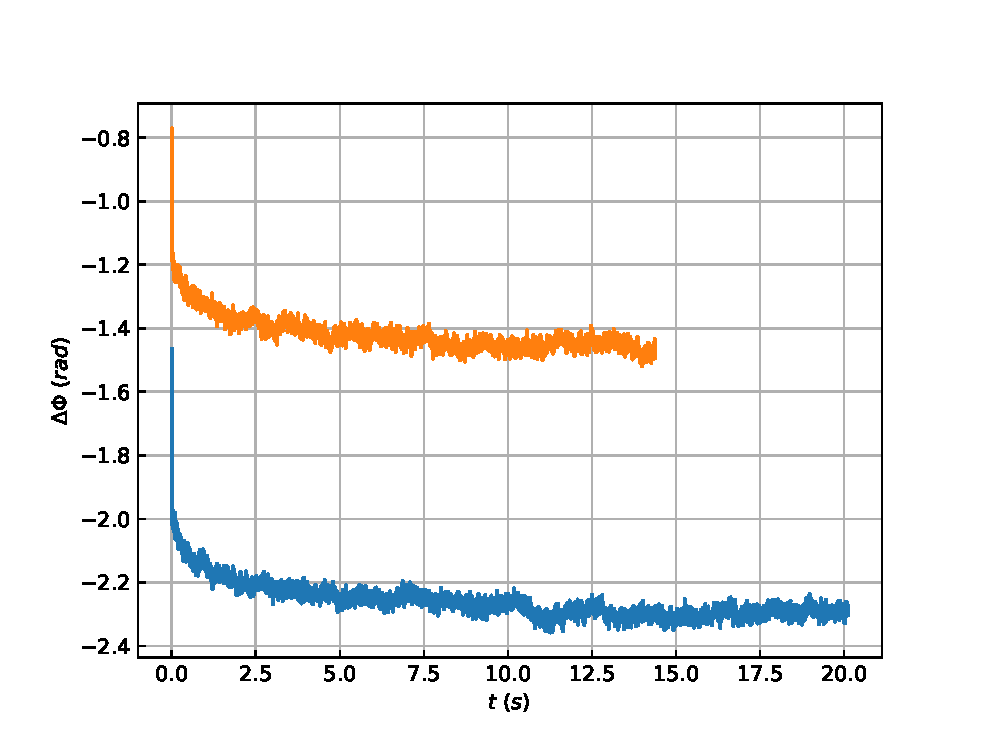
\includegraphics[scale=1.0]{drawings/phase_sync}
    \par\end{centering}
    \protect\caption{\label{fig:phase_sync_result}Fazių skirtumas tarp dviejų SDR imtuvų.}
\end{figure}

\ref{fig:phase_sync_result}~pav. galima matyti, kad fazių skirtumas tarp
imtuvų po kurio laiko nusistovi. Grafike pavaizduoti du atskiri matavimai,
matome, kad kiekvieno matavimo metu, atsiranda vis kitoks fazių skirtumas,
kaip aptarta \ref{sec:hackrf} skyriuje.
Pradėjus matavimą, fazių skirtumas nusistovi maždaug po $5\ \mathrm{s}$, tai
įtakoja kiekvieno imtuvo PLL nusistovėjimo laikas. Toks nusistovėjimas
GNSS signalų priėmimui įtakos neturės, dėl to, kad spindulio formavimas
bus pradedamas tik po kalibravimo, bei pirmų koordinačių gavimo,
kuris trunka daugiau negu $30\ \mathrm{s}$.
Iš grafiko taip pat matome, kad nusistovėjus fazei, nestebimas didelis fazių skirtumo
kitimas, iš to galime daryti išvadą, kad abu imtuvai yra sinchronizuoti tiek fazėje,
tiek dažnyje.

Norint atlikti kalibravimą, reikia gauti fazės skirtumo vidurkį, jį išsisaugoti.
Turint fazių skirtumą, jį galime taikyti kaip konstantą SDR imtuvui. Kai imtuvai
yra sinchronizuoti laike, dažnyje ir fazėje, galime taikyti spindulio formavimo
algoritmus.

\end{document}
